The two component diagrams expose how the system architecture is build at two different level of abstraction: the high level component diagram shows how the main subsystem are arranged and interconnected and what interfaces do they use to communicate; the application server component diagram instead contains a more detailed description of what software components have to be implemented within the application server subsystem.

\begin{figure}[h]
\centering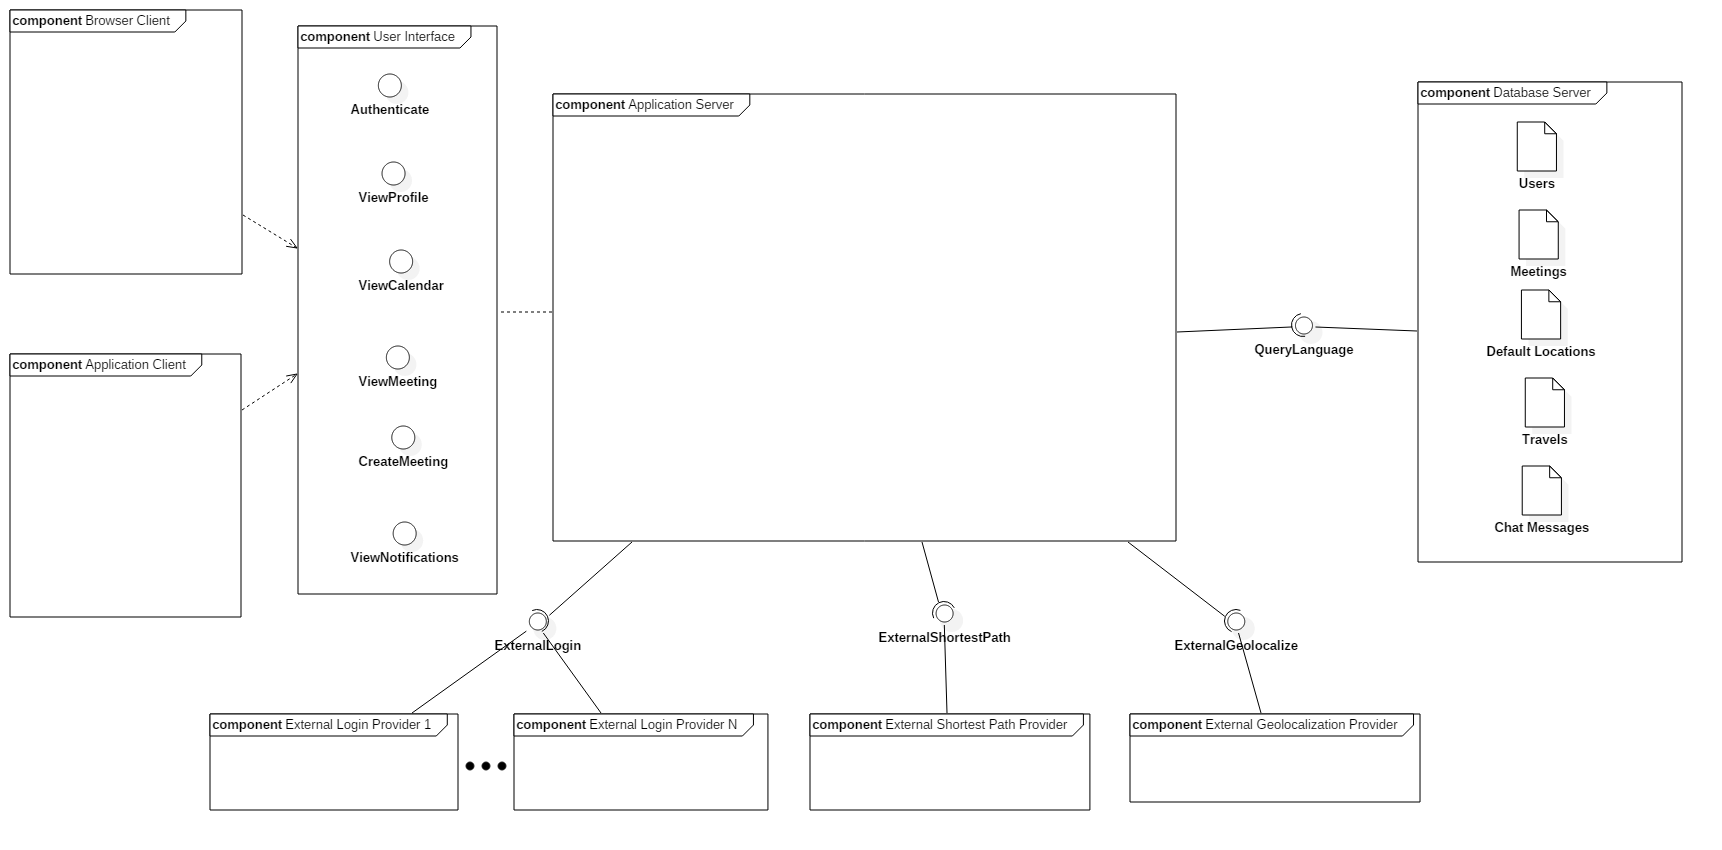
\includegraphics[width=\textwidth]{Images/UMLDiagrams/HighLevelComponentDiagram.png}
\caption{High Level Component Diagram}
\end{figure}

\begin{itemize}
\item Route Manager: manages the mapping between URLs and core system interfaces; it is the gateway for every request incoming from the clients.
\item Webpage Engine: manages the building of the web pages and the storage and retrieval of their templates.
\item Query Manager: manages the interfaces towards the storage of persistent data (i.e. the database), allowing the rest of the system to interact with them in a more abstract way.
\end{itemize}

\begin{figure}[h]
\centering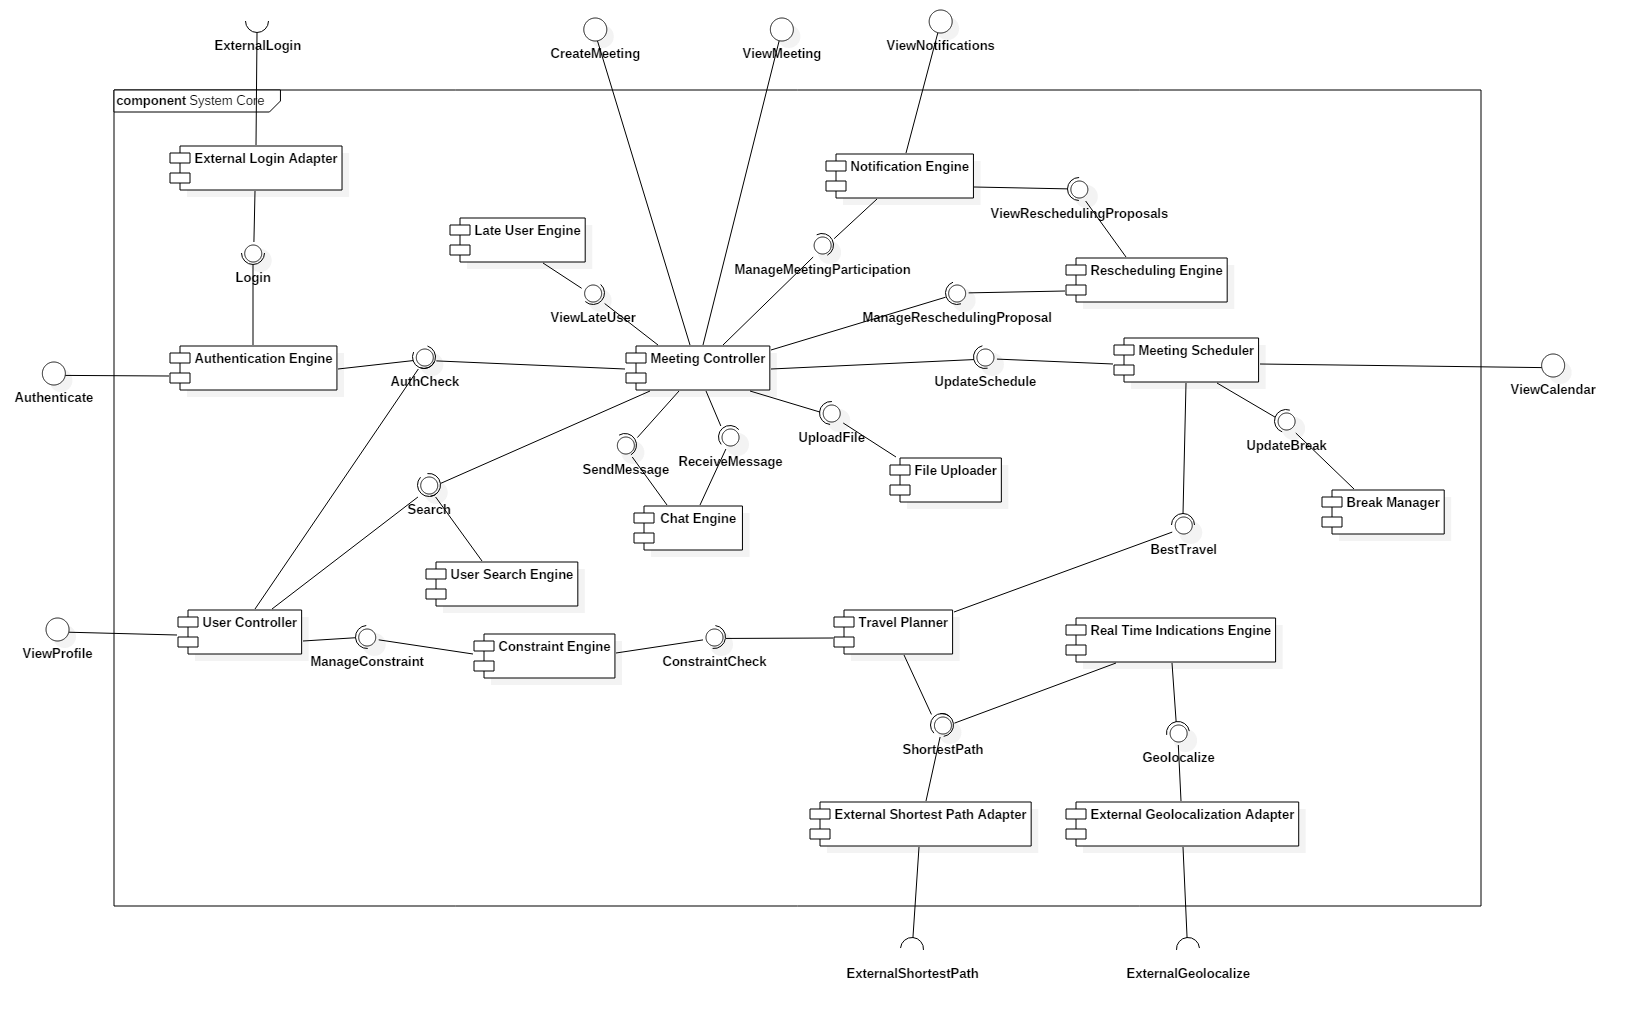
\includegraphics[width=\textwidth]{Images/UMLDiagrams/ApplicationComponentDiagram.png}
\caption{System Core Component Diagram}
\end{figure}

\begin{itemize}
\item Authentication Engine: manages everything related to registration and login and provides to the rest of the system an interface to always know if a request comes from a user and, if so, from what user.
\item External Login Adapter: manages the interface toward external login providers.
\item User Controller: manages everything related to the users, such as their profile and their settings.
\item User Search Engine: manages the search of a user in the system by some keywords, such as their email or nickname.
\item Constraint Engine: manages all the constraints available in the system and provides an interface for the user to change their ones and an interface for checking if a specific constraint has to be enforced on a specific travel.
\item Meeting Controller: manages everything related to the meetings, from the side of both the users and the administrators.
\item Chat Engine: manages the chat system present in every meeting.
\item Late User Engine: uses the data about the positions of the users to extrapolate who's late for any meeting and created a dashboard for the administrator to visualize it.
\item File Uploader: manages the upload of files for the meetings.
\item Travel Planner: computes the best travel between two given locations for a given user.
\item Real-Time Indications Engine: manages the real-time indications given to a user to guide him towards its next meeting.
\item External Shortest Path Adapter: manages the interface toward external shortest path providers.
\item External Geolocalization Adapter: manages the interface towards external geolocalization providers.
\item Meeting Scheduler: manages the users' schedules and the insertions of new meetings into it.
\item Break Manager: manages the flexible breaks and upload their effective time whenever it's needed.
\item Rescheduling Engine: manages the rescheduling proposal for the meetings and their responses.
\item Notification Engine: manages all the notifications that are sent to the users, such as warnings and meeting invitations.
\end{itemize}